\chapter{Modeling} \label{ch:modeling}

This chapter is concerned with the mathematical model of the wheeled robotic vehicle and will serve as a pre-requisite for the later implemented feedback control algorithm. 
The dynamics part, describing the motor model, will be used in the cruise control derivation. Subsequently the kinematics model, which treats the robot as a point entity, will be used in the estimation for position control.

\section{Differential Drive} \label{kin_model} 

Differential drive steering, a popular choice in mobile robots, is a design where two wheels on a same axle are controlled independently. It may or may not include a castor wheel, however this paper addresses the latter. Depending on the relative rotation of each wheel, the robot could be steered in a desired manner. For the sake of clarity, several basic cases of interest are presented along with the equations describing the linear and angular velocity of the vehicle. 

\begin{align}
v = \frac{Rw_r + Rw_l}{2} \label{eq1} \\
W = \frac{Rw_r - Rw_l}{l} \label{eq2} 
\end{align}

Equation \ref{eq1} describes the linear speed of the robotic vehicle, with respect to the angular speeds of each wheels (\textbf{$w_r$}) and (\textbf{$w_l$}) and the wheel radius (\textbf{R}), while \ref{eq2} describes the angular speed of the robot, with \textbf{l} being the axle length between the wheels. 
The equation could be rewritten in matrix form as:

\begin{equation}  	\label{eq3} 
\begin{pmatrix}
	v \\
	\omega	
\end{pmatrix} 
=
\begin{pmatrix} 
	\frac{R}{2} & \frac{R}{2} \\
	\frac{R}{l} & \frac{-R}{l} 
\end{pmatrix}
\begin{pmatrix}
	\omega_r \\
	\omega_l
\end{pmatrix}  	
\end{equation}

Analysis of the above equation leads to the consideration of three cases where certain behaviour is to be expected.

\begin{itemize} \label{list_v}

\item $\boldsymbol{v_r = v_l}$ \\ In this case scenario, both wheels have the same speed. The robot's speed from equation \ref{eq13} is simply equal to the individual speed of each of wheel. On the other hand, the angular speed from equation \ref{eq14} becomes 0, and the turning radius infinite. The robot is expected to perform straight linear motion.

\item $\boldsymbol{v_r = 0}$ or $\boldsymbol{v_l = 0}$ \\ In this case scenario, the turning radius becomes $\frac{l}{2}$. The robot is expected to perform rotation either about the right or the left wheel, with the center of rotation being the zero velocity wheel. 

\item $\boldsymbol{v_l = -v_r}$ \\ In this case scenario, the turning radius and the linear speed become 0, while the angular speed is doubled. The robot is expected to perform rotation about it's midpoint, or simply put in-place rotation.

\end{itemize}

\subsection{Non-holonomic constraints} 

A robot, using the differential drive steering design, has restricted local movements, while having no restrictions in global motion. \todo{Reference} That is similar to the restrictions on a car, where it is not possible to slide into a parallel position with respect to the current one. Nevertheless, the vehicle can still manoeuvre into the desired position, similar to parallel parking. 

If we consider \todo{insert vehicle figure} we can define the non-holonomic constraints of a differential drive vehicle as: 

\begin{equation} \label{eq4}
\dot{x}sin(\theta) - \dot{y}cos(\theta) = 0
\end{equation}

As observed from equation \ref{eq4} and shown by figure \ref{fig::xy_orient}, the robot can not have speed perpendicular to the sagittal axis. The equation can be further rewritten as:

\begin{equation} \label{eq5} 
\tan{\theta} = \frac{\dot{y}}{\dot{x}} = \frac{dy}{dx}
\end{equation} 
\\

\begin{figure}[h]
\centering
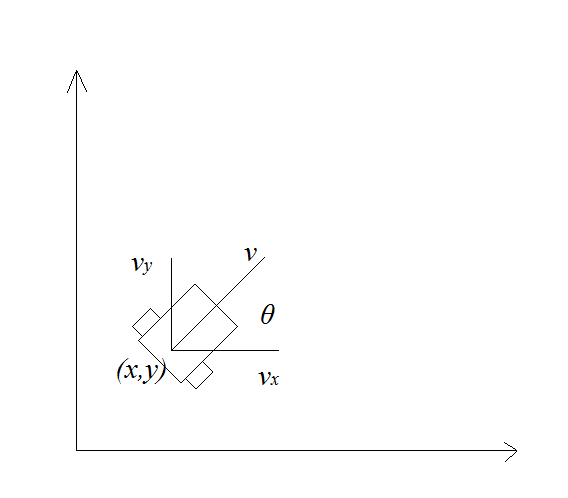
\includegraphics[width=0.5\textwidth]{Orientation_xy}
\caption{WMR orientation}
\label{fig::xy_orient}
\end{figure}

\section{Kinematics} \label{kinematics}

The kinematic model, similar to most rigid vehicles travelling on a two-dimensional plane, is of three degrees of freedom. From figure \ref{fig::xy_orient}, we can identify \textbf{x} and \textbf{y} as the coordinates for the center of mass of the robot and \textbf{$\theta$} as the angle with respect to the x axis. From the constraints of the vehicle, the equations concerning the kinematic model are derived as:

\begin{align}
\dot{x} = vcos(\theta) \nonumber \\
\dot{y} = vsin(\theta) \label{eq6} \\
\dot{\theta} = \omega  \nonumber 
\end{align}

Where \textbf{v} is the linear and \textbf{$\omega$} is the angular speed of the vehicle.
The equations could further be represented in matrix form.

\begin{equation} \label{eq7} 
\begin{pmatrix}
	\dot{x} \\
	\dot{y} \\
	\dot{\theta} \\ 
\end{pmatrix} 
=
\begin{pmatrix} 
	\cos{\theta} & 0 \\
	\sin{\theta} & 0 \\
	0     		 & 1  
\end{pmatrix}
\begin{pmatrix}
	v \\
	\omega
\end{pmatrix}  	
\end{equation}


%The relation between the linear speed and the angular speed of the robot is similar to equation \ref{eq12}.

%\begin{equation} \label{eq15} 
%v = WD
%\end{equation}

%Where D is the turning radius, from the midpoint of the wheels to the ICC. Solving for the turning radius, yields:

%\begin{align}
%D = \frac{v}{W} \label{eq16} \\
%= \frac{l}{2}\frac{v_r + v_l}{v_r - v_l} \nonumber
%\end{align}

\section{Dynamics} \label{dc_math}

%\begin{figure}[h] %change image
%\centering
%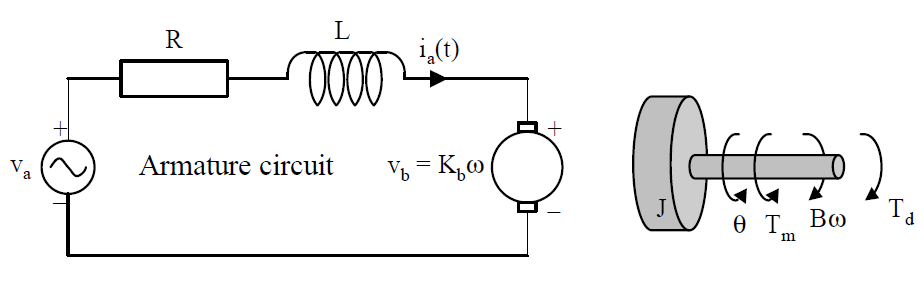
\includegraphics[width = 0.7\textwidth]{Motor_curcuit}
%\caption{Electrical circuit and free-body diagram of DC motor \cite{FBD}}
%\label{fig::motor_curcuit}
%\end{figure} 

In this section the equations used in the dynamics model of the motor are derived and described.

A DC motor produces mechanical torque applied to the shaft($\boldsymbol{T_e}$) linearly proportional to the armature current, the magnetic field and a torque constant($\boldsymbol{K_t}$). Assuming constant magnetic field, the produced torque is proportional to the torque constant($\boldsymbol{K_t}$) and the armature current(\textbf{I}).( Equation \ref{eq1})Furthermore, the back Emf (electromotive force)($E_b$) is equal to the angular velocity($\omega$) of the shaft multiplied with the Back emf constant($K_b$).(Equation \ref{eq2}) \\

\begin{align}  
T_e = IK_t \label{eq8}\\
E_b = \omega K_b \label{eq9}
\end{align}

Because the two constants $K_t$ and $K_b$ are equal in SI units, in further equations and simulations they will be denoted only as a motor constant $K$.

%VERIFY AND MODIFY

%\begin{equation} \label{eq3}
%K_t = K_b = K
%\end{equation} 

Using Kirchhoff's voltage law, the equations modelling the electrical part of the DC motor are derived as:

\begin{equation} \label{eq10}
V = RI + L\frac{dI}{dt} + E_b
\end{equation} 

where (\textbf{V}) is the applied voltage, (\textbf{R}) the armature resistance,(\textbf{L}) the armature inductance, ($\boldsymbol{E_b}$) the Back EMF. \ref{eq4}
Substitution ($\boldsymbol{E_b}$) with \ref{eq8} yields:

\begin{equation} \label{eq11}
V = RI + L\frac{dI}{dt} + K_b\omega
\end{equation}

The mechanical part of the DC motor(mechanical part of figure \ref{fig::motor_curcuit}) is described by Newton's second law for rotational motion as:

\begin{equation} \label{eq12}
J\dot{\omega} = K_tI - b\omega
\end{equation}

Where \textbf{J} is the load's inertia and \textbf{b} is the viscous friction in the motor's bearings.
Further substitution in equation \ref{eq4} with the derived back emf from \ref{eq2} results in:

Equations \ref{eq10} and \ref{eq11} are the equations describing the electrical and mechanical part of the motor.

Applying the Laplace transform to the equations \ref{eq10} and \ref{eq11}, we can relate the output angular velocity to the input voltage as described in the transfer function:

\begin{equation} \label{eq13}
\frac{\Omega(s)}{V(s)} = \frac{K_t}{(Js + b)(sL + R) + K_tK_b}
\end{equation}

The state space form representation of equations \ref{eq10} and \ref{eq11} is represented in the form $\dot{x} = Ax + Bu$ , where the state variables are the current (\textbf{I}) and the angular speed ($\boldsymbol{\omega}$)

\begin{equation} \label{eq14} 
\begin{pmatrix}
	\dot{I} \\
	\dot{\omega} \\
\end{pmatrix} 
=
\begin{pmatrix} 
	\frac{-b}{J}   & \frac{-K_t}{J} \\
	\frac{-K_b}{L} & \frac{-R}{L} \\ 
\end{pmatrix}
\begin{pmatrix}
	I \\
	\omega
\end{pmatrix}
+
\begin{pmatrix}
	\frac{1}{L} \\
	0
\end{pmatrix}
V	
\end{equation}


The Simulink block diagram describing the behaviour of the DC motor in continuous time is given in figure \ref{fig::motor_block}.

\begin{figure}[h]
\centering
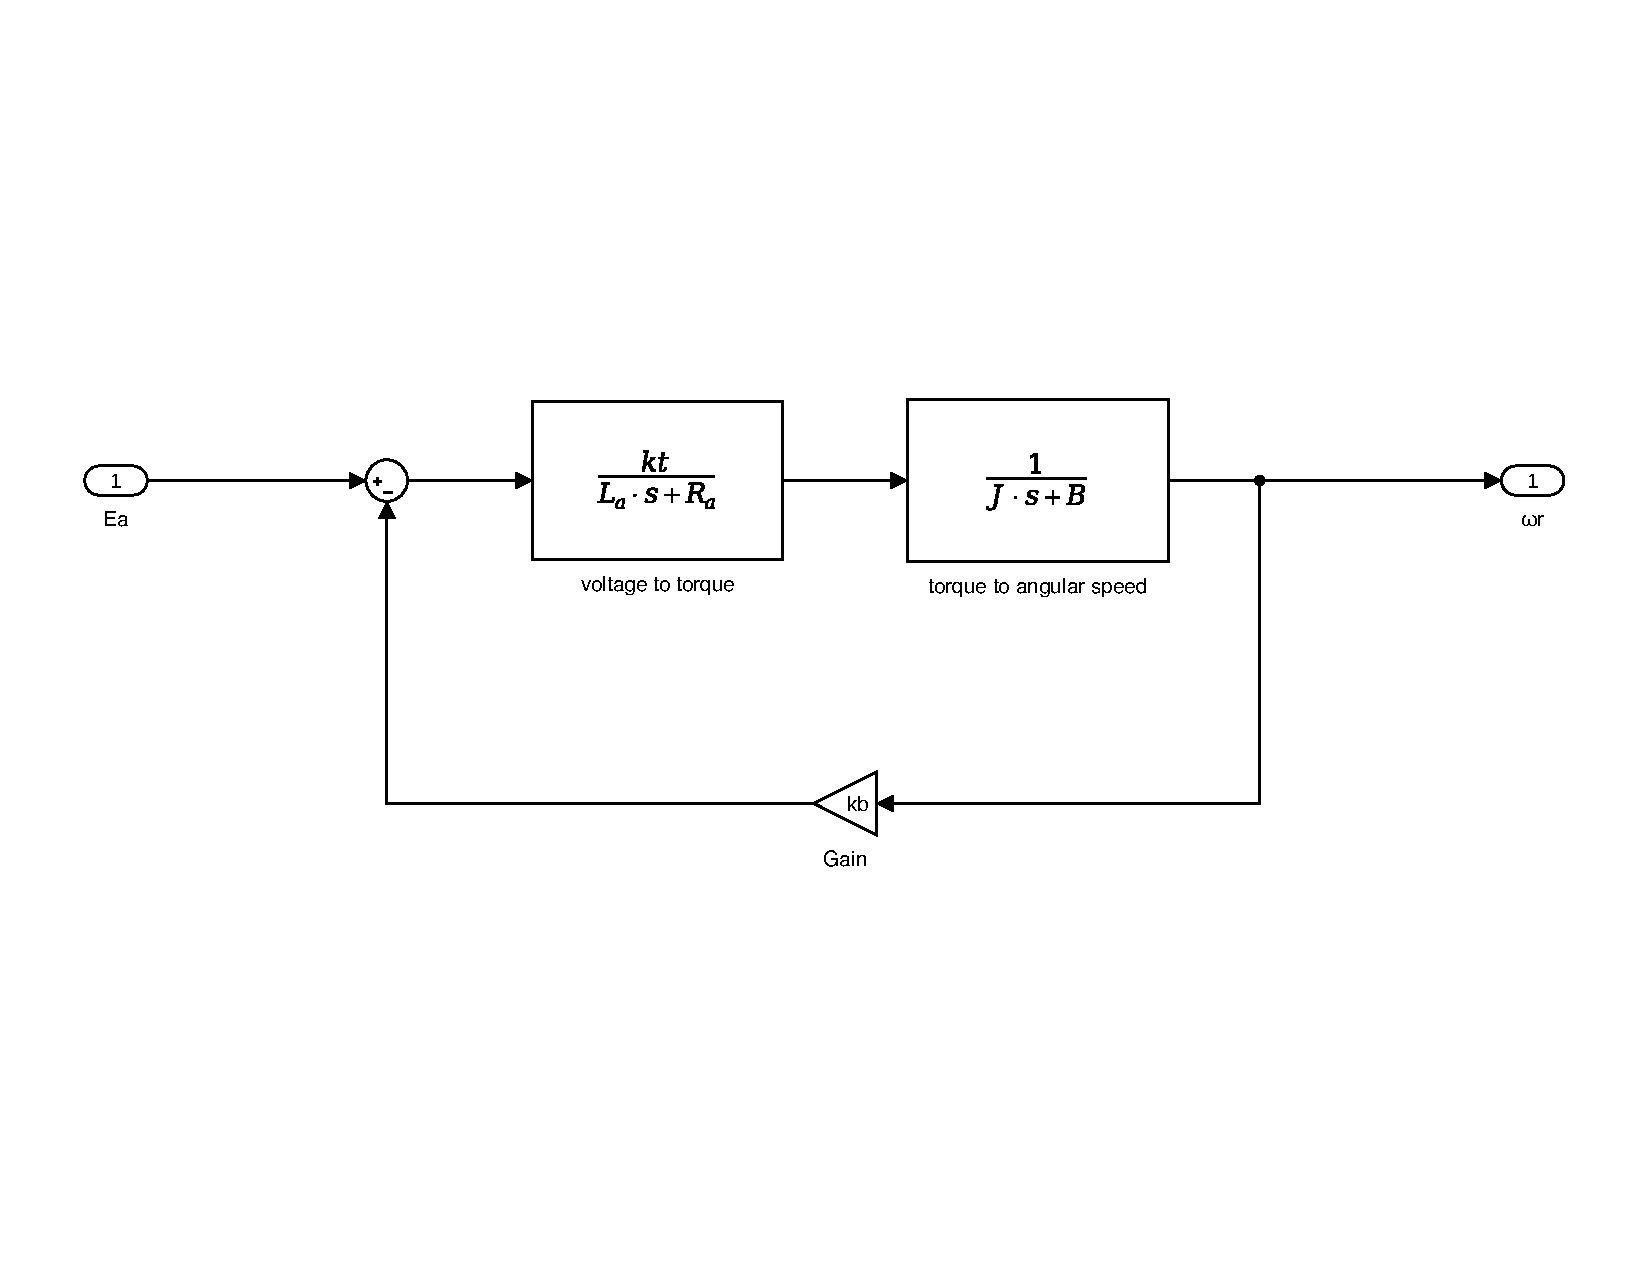
\includegraphics[width=0.5\textwidth]{dcmodel}
\caption{Motor block diagram}
\label{fig::motor_block}
\end{figure}

The motor model is a SISO system, where the input is Voltage and the output is angular velocity. Thus, classical control is sufficient to manipulate the behaviour of the system.  

\section{Complete Model} 

Combining the motor dynamics, the the robot kinematics yield the complete plant of the system.

\section{Dead reckoning} 

If we consider the robot's configuration \textbf{q}, previously described as (x,y,$\theta$), a way of measuring the above mentioned configuration is required in order to implement planning and feedback control. Incremental encoders are common in wheeled robots as they are able to measure the rotation of the wheels. However, they do not provide direct measurements of the position and orientation of the robot, thus dead reckoning (aka. odometric localization) is an affordable way to estimate the vehicle's configuration \textbf{q} by iterative integration of the kinematic model from \ref{kinematics}. The major drawback of the method is the proneness to error, that is if there exists a small error in any step of the localization it will influence the calculation of the subsequent positions, leading to potentially large deviation between the expected position and the localization results. From that we can conclude that dead reckoning is less precise in large areas due to systematic errors( eg. limited encoder resolution, unequal wheel diameters, etc.), and external factors not considered in the kinematics due to non-systematic errors( eg. wheel slippage on floors, inclined surfaces etc.) \todo{ref book Modelling.Planning and Control}

Assuming constant inputs $\boldsymbol{v_k}$ and $\boldsymbol{\omega_k}$ in the kinematic model \ref{kinematics} for discrete time [$t_k$,$t_{k+1}$] (zero-order hold), for the sampling step \textbf{k} =1,2,...,n, the differential drive robot will traverse along an arc with a circle radius \textbf{D} ($\frac{v_k}{\omega_k}$). Furthermore if the starting position ($x_k$,$y_k$,$\theta_k$), for \textbf{k} =1, and the velocities $\boldsymbol{v_k}$ and $\boldsymbol{\omega_k}$ are known, we can reconstruct the value of ($x_{k+1}$,$y_{k+1}$,$\theta_{k+1}$) by forward integration of the kinematic model at the sampling time $t_{k+1}$. Several methods for numerical integration could be used, among which are the Forward Euler method, Second-order Runge-Kutta method or exact integration. \todo{ref Robotics book}. Because of inadequate accuracy due to the constant orientation $\theta_k$ in the Euler method, in this paper we will consider the Runge-Kutta approximation method and exact integration as described in the book "Robotics: Modelling, Planning and Control" by Bruno Siciliano.

\begin{align}
x_{k+1} = x_k + T_s v_k cos(\theta_k + \frac{\omega_k T_s}{2}) \\
y_{k+1} = y_k + T_s v_k sin(\theta_k + \frac{\omega_k T_s}{2}) \label{eq15} \\
\theta_{k+1} = \theta_k + T_s\omega_k  \nonumber 
\end{align}

Equation \ref{eq15} refers to the second-order Runge-Kutta method, where $\boldsymbol{T_s}$ is the duration of the sampling period $T_s = t_{k+1} - t_k$. It is important to note that the approximations for $x_{k+1}$ and $y_{k+1}$ use the average value of the unicycle orientation in the sampling period, compared to the less accurate Euler method with constant orientation.

The exact reconstruction of ($x_{k+1}$,$y_{k+1}$,$\theta_{k+1}$), assuming constant velocity inputs in the sampling interval is given by \ref{}:\todo{reference to book} 

\begin{align}
x_{k+1} = x_k + \frac{v_k}{\omega_k}(sin(\theta_{k+1} - sin(\theta_k)\\
y_{k+1} = y_k + \frac{v_k}{\omega_k}(cos(\theta_{k+1} - cos(\theta_k) \label{eq16} \\
\theta_{k+1} = \theta_k + T_s\omega_k  \nonumber 
\end{align}

Note that the exact reconstruction is not defined for $w_k$ = 0 (motion in a line segment) thus, in implementation, a conditional statement has to handle the exception by using the Runge-Kutta method, which is still defined for $w_k$ = 0.

Nevertheless, in practice it is convenient to estimate the input velocities using the incremental encoders	and by calculating the relative displacement $\Delta s$ and orientation $\Delta\theta$  over the sampling period:

\begin{align}
v_k T_s = \Delta s \nonumber \\
\omega_k T_s = \Delta\theta \label{eq17} \\
\frac{v_k}{\omega_k} = \frac{\Delta s}{\Delta\theta} \nonumber
\end{align}

In the case of a differential drive robot with a castor wheel, from equation \ref{eq1} and \ref{eq2}, we can define $\Delta s$ and $\Delta\theta$ as :

\begin{align}
\Delta s 	 = \frac{r}{2}(\Delta s_r + \Delta s_l) \label{eq18} \\
\Delta\theta = \frac{r}{l}(\Delta s_r - \Delta s_l) \nonumber
\end{align}

Where $\Delta s_r$ and  $\Delta s_l$ are the rotation of the right and left wheel, respectively, measured by the incremental encoders during the sampling period. 


\section{System Parameters} \label{parameter}

In this section the parameters used in the mathematical model of the robot are given. They were acquired by measurements and experiments on the physical system, prior to implementation.

\begin{table}[h]
\centering
\begin{tabular}{cccll}
\hline
Parameter                   & Description                               & Nominal Value                                 &  &  \\ \hline
\multicolumn{1}{|c|}{K}     & \multicolumn{1}{c|}{Motor constant}       & \multicolumn{1}{c|}{0.1838 V/(rad/s)  Nm/amp} &  &  \\ \cline{1-3}
\multicolumn{1}{|c|}{R}     & \multicolumn{1}{c|}{Armature resistance}  & \multicolumn{1}{c|}{11.5 $\Omega$}            &  &  \\ \cline{1-3}
\multicolumn{1}{|c|}{L}     & \multicolumn{1}{c|}{Armature inductance}  & \multicolumn{1}{c|}{0.1 H}                    &  &  \\ \cline{1-3}
\multicolumn{1}{|c|}{$b_r$} & \multicolumn{1}{c|}{Rotor damping}        & \multicolumn{1}{c|}{0.0221}                   &  &  \\ \cline{1-3}
\multicolumn{1}{|c|}{$J_w$} & \multicolumn{1}{c|}{Load inertia} & \multicolumn{1}{c|}{2.8033e-5 $KgM^2$}        &  &  \\ \cline{1-3}
\multicolumn{1}{|c|}{n}     & \multicolumn{1}{c|}{Gear ratio}           & \multicolumn{1}{c|}{1:48}                     &  &  \\ \cline{1-3}
\multicolumn{1}{l}{}        & \multicolumn{1}{l}{}                      & \multicolumn{1}{l}{}                          &  &  \\ \hline
\end{tabular}
\caption{System parameters}
\label{sys_par}
\end{table}

\todo{include all parameters} 

 